\documentclass{article}

\usepackage{amsmath}
\usepackage{amssymb}
\usepackage{float}
\usepackage{graphicx}
\usepackage{geometry}
\geometry{a4paper, margin=1in}

\title{Convolution of \( f(t) = \log t \) with a Rectangular Kernel}

\begin{document}

\maketitle

\section{Problem Statement}

Compute the convolution of the signal \( f(t) = \log t \) with the rectangular kernel:
\[
h(t) =
\begin{cases}
1, & -T \leq t \leq T \\
0, & \text{otherwise}
\end{cases}
\]

The convolution is defined as:
\[
y(t) = (f * h)(t) = \int_{-\infty}^{\infty} f(\tau) h(t-\tau) \, d\tau
\]

We also analyze the system behavior for various values of \( T \), and consider modified and shifted kernels.

\section*{Derivation of \( y(t) \)}

Since \( h(t-\tau) \) is nonzero only when \( -T \leq t-\tau \leq T \), it follows that:
\[
t-T \leq \tau \leq t+T
\]
Thus, the convolution becomes:
\[
y(t) = \int_{t-T}^{t+T} \log \tau \, d\tau
\]

Using the integral:
\[
\int \log \tau \, d\tau = \tau \log \tau - \tau + C
\]
we obtain:
\[
y(t) = \left[ \tau \log \tau - \tau \right]_{t-T}^{t+T}
\]
Expanding:
\[
y(t) = (t+T)\log(t+T) - (t+T) - (t-T)\log(t-T) + (t-T)
\]
Simplifying:
\[
\boxed{y(t) = (t+T)\log(t+T) - (t-T)\log(t-T) - 2T}
\]
\newpage
\section*{Behavior Analysis for Different \( T \)}
\textbf{Near \( t=0 \)}: \( \log 0 \) is undefined; restrict domain to \( t > T \).
\begin{itemize}
    \item \textbf{Small \( T \)}: Localized smoothing around \( t \). Mean squared error between analytical and simulated plots: 0.00206248319793766
    \begin{figure}[H]
    \centering
    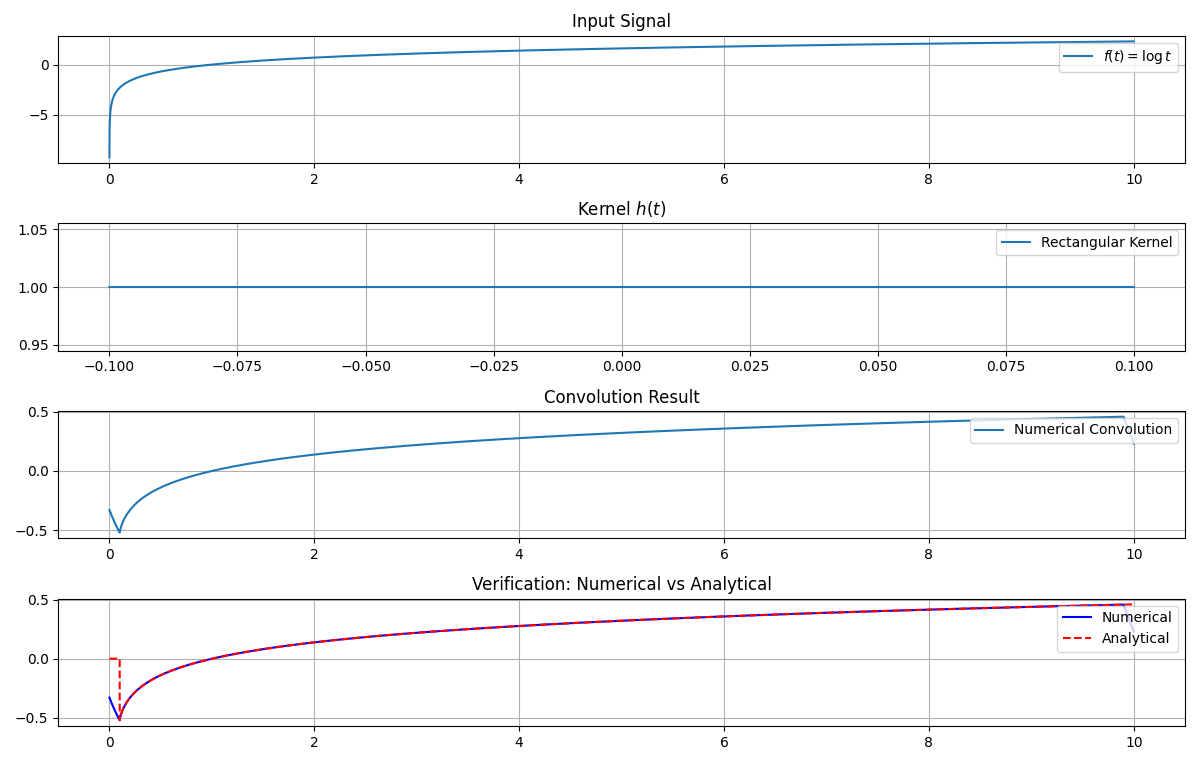
\includegraphics[width=1\textwidth]{2.png}
    \end{figure}
    \item \textbf{Large \( T \)}: Broad averaging, heavy smoothing. Mean squared error between analytical and simulated plots: 0.14497976045750576
    \begin{figure}[H]
    \centering
    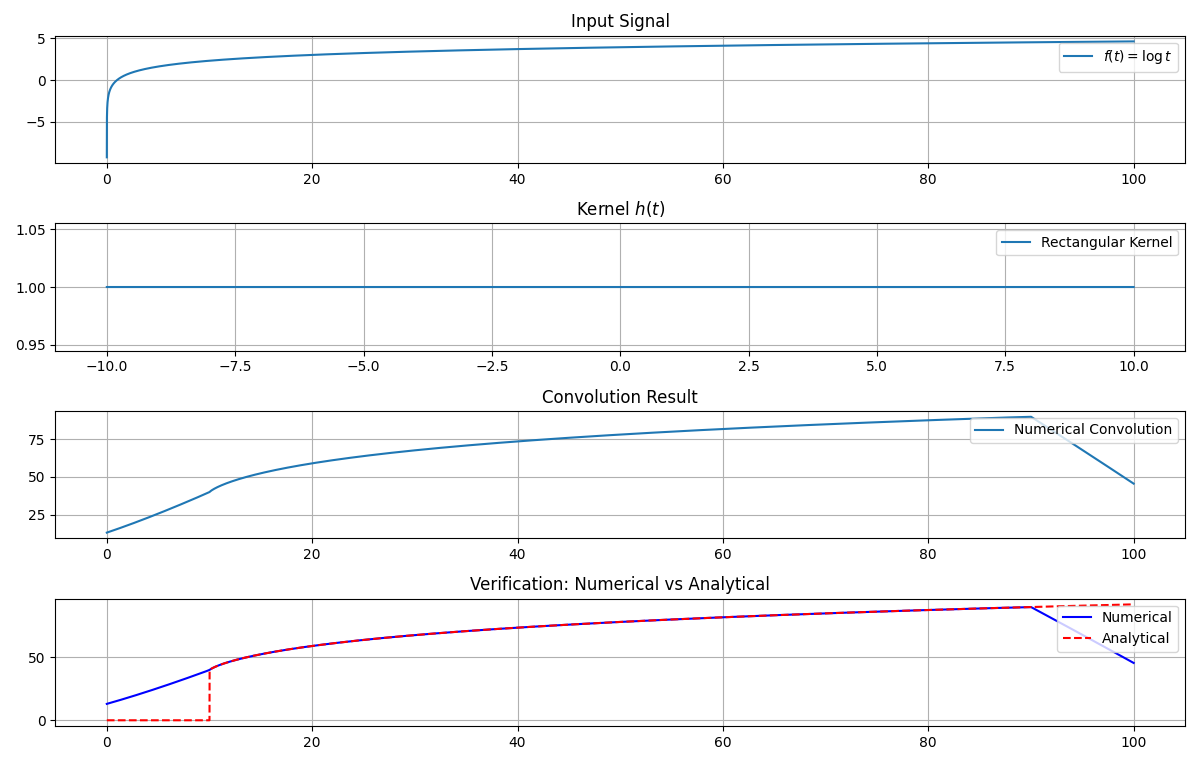
\includegraphics[width=1\textwidth]{1.png}
    \end{figure}
   
\end{itemize}

\section*{Modifications}

\subsection*{(a) Kernel Considering Only \( t>0 \)}

Modified kernel:
\[
h(t) =
\begin{cases}
1, & 0 \leq t \leq T \\
0, & \text{otherwise}
\end{cases}
\]

Nonzero range:
\[
t-T \leq \tau \leq t
\]

Thus:
\[
y(t) = \int_{t-T}^{t} \log \tau \, d\tau
\]

Evaluating:
\[
y(t) = \left[ \tau \log \tau - \tau \right]_{t-T}^{t}
\]
\[
y(t) = t\log t - t - (t-T)\log(t-T) + (t-T)
\]
Simplifying:
\[
\boxed{y(t) = t\log t - (t-T)\log(t-T) - T}
\]

\textbf{Impact:} The system becomes \textit{causal}, depending only on past values.

\subsection*{(b) Shifted Kernel by \( \tau_0 \)}

Shifted kernel \( h(t-\tau_0) \) is nonzero when:
\[
\tau_0-T \leq t \leq \tau_0+T
\]

In convolution:
\[
y(t) = \int_{t-\tau_0-T}^{t-\tau_0+T} \log \tau \, d\tau
\]

Evaluating:
\[
y(t) = \left[ \tau \log \tau - \tau \right]_{t-\tau_0-T}^{t-\tau_0+T}
\]
\[
y(t) = (t-\tau_0+T)\log(t-\tau_0+T) - (t-\tau_0+T) - (t-\tau_0-T)\log(t-\tau_0-T) + (t-\tau_0-T)
\]
Simplifying:
\[
\boxed{y(t) = (t-\tau_0+T)\log(t-\tau_0+T) - (t-\tau_0-T)\log(t-\tau_0-T) - 2T}
\]

\textbf{Impact:} Introducing a shift \( \tau_0 \) causes a \textit{time delay} in the output.

\section*{Summary}

\begin{itemize}
    \item Original convolution averages symmetrically.
    \item Modified kernel (\( t>0 \)) yields a causal system.
    \item Shifting the kernel results in delayed outputs, significant in time-delayed systems.
    \item Care must be taken near \( t=0 \) due to \( \log 0 \) being undefined.
\end{itemize}

\end{document}
